Although the evolution of star formation rate density (SFRD) and black
hole accretion rate (BHAR) with redshift track each other at
$z\lesssim3$, it is unclear whether this is true at higher redshift,
$z\gtrsim4$. Indeed recent studies (e.g. Khostovan et al., 2015, MNRAS
452, 3948; Vito et al., 2018, MNRAS 473, 2378; Calhau, Sobral et
al. 2018, MNRAS in prep.)  suggest not. Here we aim to examine the
$z\sim5$ quasar population in order to understand in great detail the
systems of the hosts of massive active black holes at a key epoch of
SMBH mass build-up $\approx$0.85-1.2 Gyr after the Big Bang.

\smallskip
\smallskip
\noindent
Our latest studies show that there is a population of 
$z=5-6.5$ quasars which are  bright in WISE W3 and W4 bands ($\sim 7.5 - 17\mu$m 
and 20-27$\mu$m) and we aim to get moderate-to- high-resolution spectra across the full 
wavelength coverage of JWST. The NIRSpec Fixed Slit configuration has a 
$R\sim2700$ across 0.81-5.14$\mu$m, and the MIRI MRS 4.9-28.5$\mu$m, 
correspoding to 0.135-4.74$\mu$m observed at $z=5$; 0.108 - 3.80$\mu$m at $z=6.5$. 

\smallskip
\smallskip
\noindent
Our main science goals would be:
\begin{itemize}
\item Build-up of the BH mass via black mass measurements (though with a decent think exactly 
       which e.g. emission lines to use; but you do have some very interesting NIR lines to work with); 
\item SFRs in the $z=5-6.5$ QSOs;
\item potential search for extended gas halos using the IFU imaging MRS mode; 
\item extending the redshift-base of BH/QSO studies given the $z>6.7$ QSO GTO time. 
\end{itemize}



\smallskip
\smallskip
\noindent
And this project would {\it highly complement} the GTO studies of the $z\geq6.7$ luminous 
quasars, as well as sample the high-mass, high-luminosity end of the Deep Field studies. 


\hspace{-7.5cm}
\begin{figure}[h]
  \begin{center}
    \hspace{-0.5cm}
%    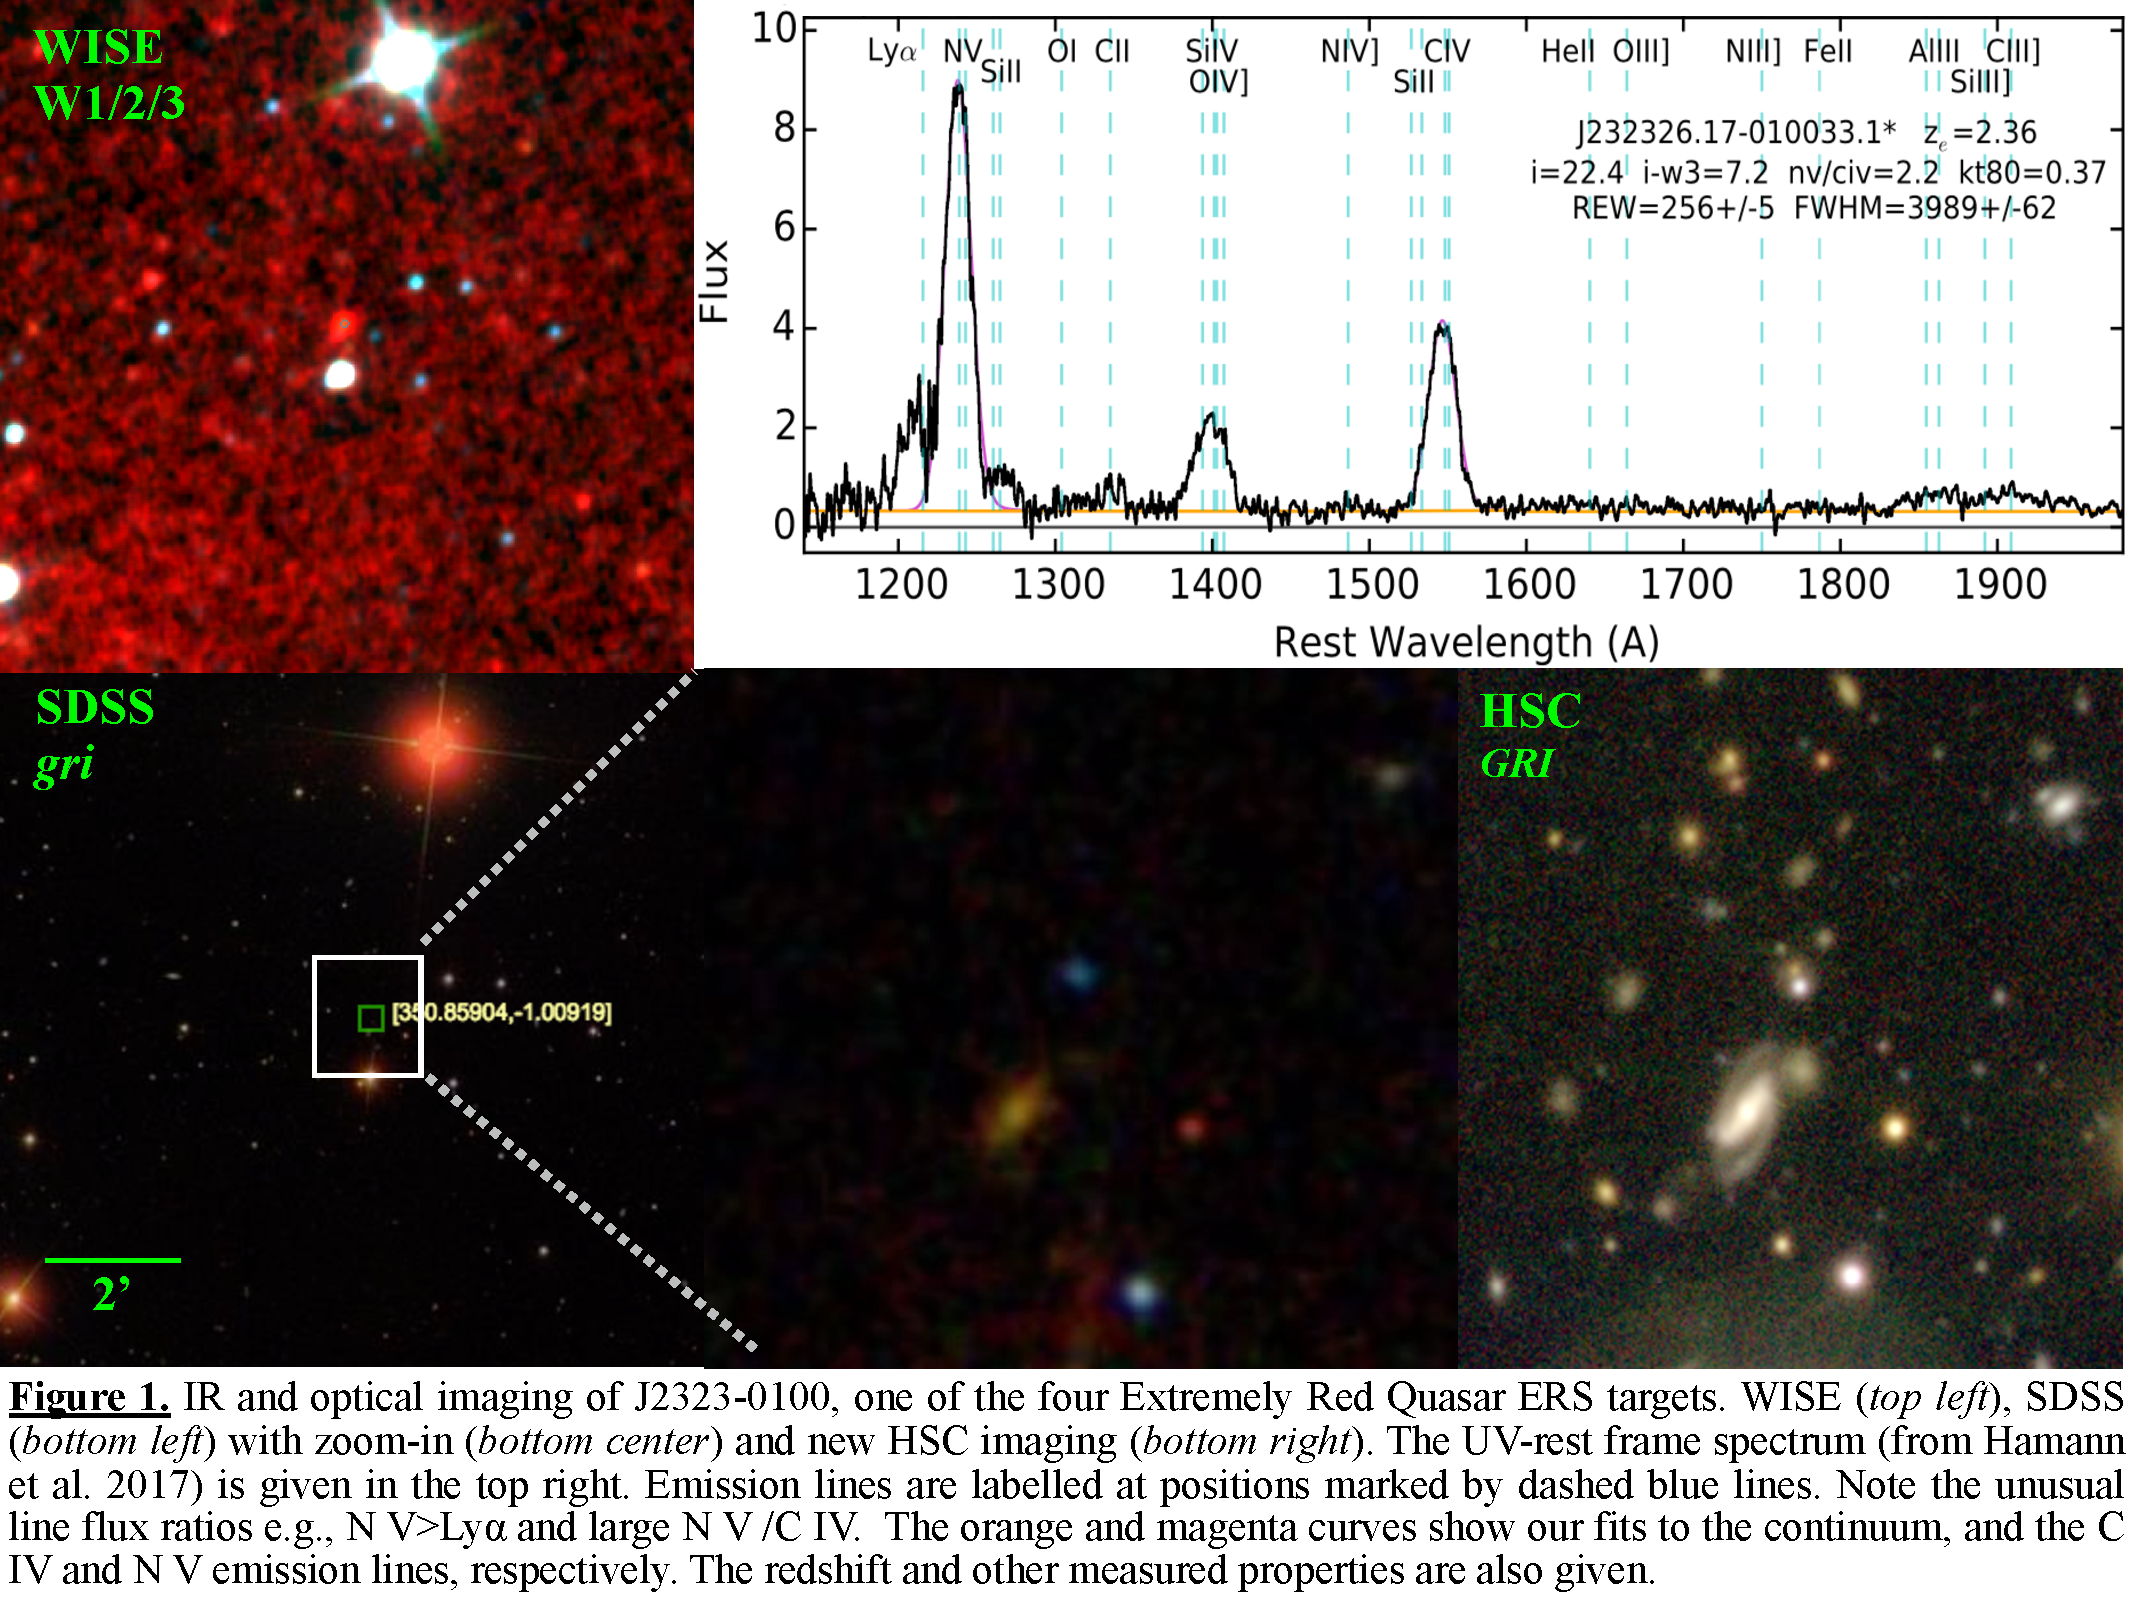
\includegraphics[]{WISE_SDSSzoomHSC_ERQ-image_v2.pdf}
    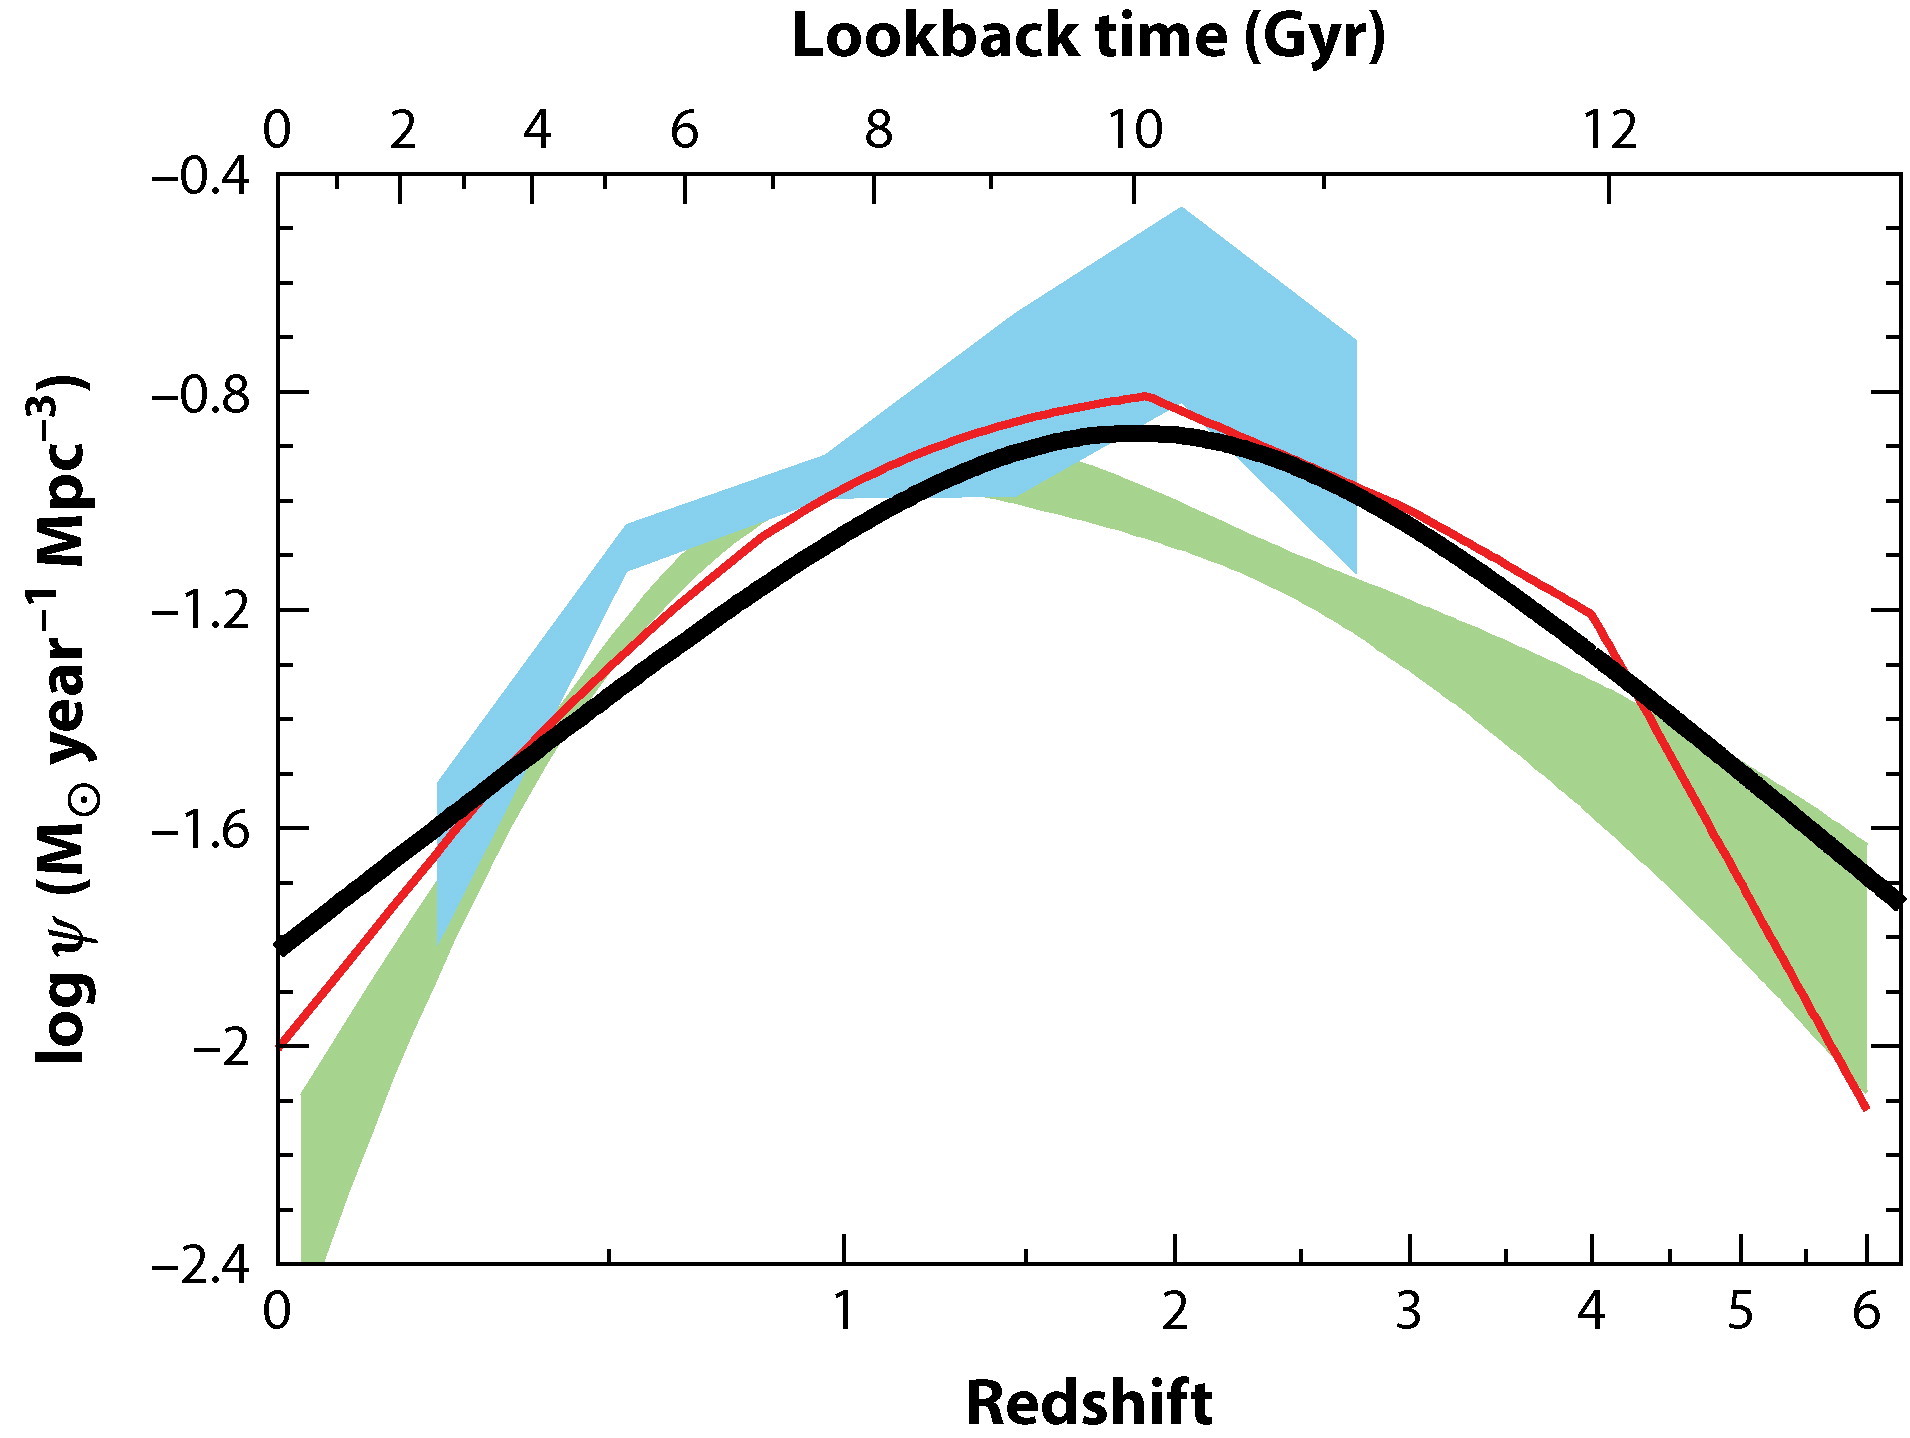
\includegraphics[height=12.0cm,width=16.0cm]{../Figures/MadauDickinson2014_Fig15_hires.jpeg}
    \vspace{-10pt}
\caption{Figure 15 from Madau \& Dickinson (2014):   
 Comparison of the best-fit star-formation history (thick solid curve)
with the massive black hole accretion history from X-ray [red curve
(Shankar et al. 2009); light green shading (Aird et al. 2010)] and
infrared (light blue shading) (Delvecchio et al. 2014) data. The
shading indicates the $\pm1\sigma$ uncertainty range on the total
bolometric luminosity density. The radiative efficiency has been set
to $\epsilon = 0.1$. The comoving rates of black hole accretion have been
scaled up by a factor of 3,300 to facilitate visual comparison to the
star-formation history.}
    \label{figtest-fig}
  \end{center}
\end{figure}

